% -*- TeX-master: "main"; fill-column: 72 -*-

\subsection{The \FBC \class{UserDefinedConstraint} class}
\label{userdefinedconstraint-class}

\newtxt{The \FBC \UserDefinedConstraint class is derived from \SBML \SBase and inherits \token{metaid} and \token{sboTerm}, as well as the subcomponents for \Annotation and \Notes. It's purpose is to allow the definition of non-stoichiometric constraints, that is, constraints that are not defined by the stoichiometrically coupled reaction network. In order to achieve this a new class of constraint is defined, the \UserDefinedConstraint.}
%
\begin{figure}[ht]
  \centering
  % Requires \usepackage{graphicx}
  %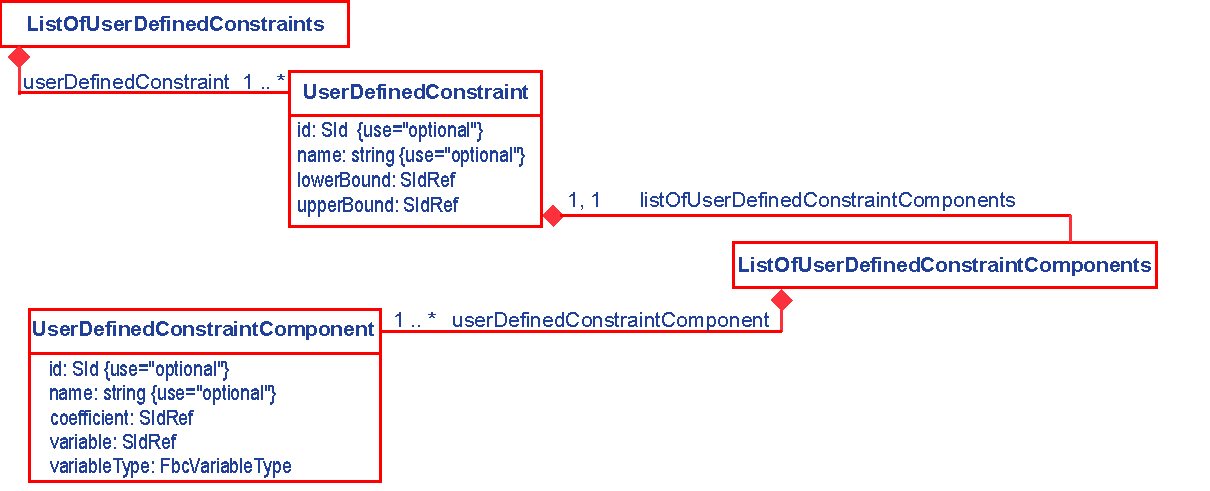
\includegraphics[width=6cm]{images/fbc_v3_uml_userdefinedconstraint.pdf}\\
  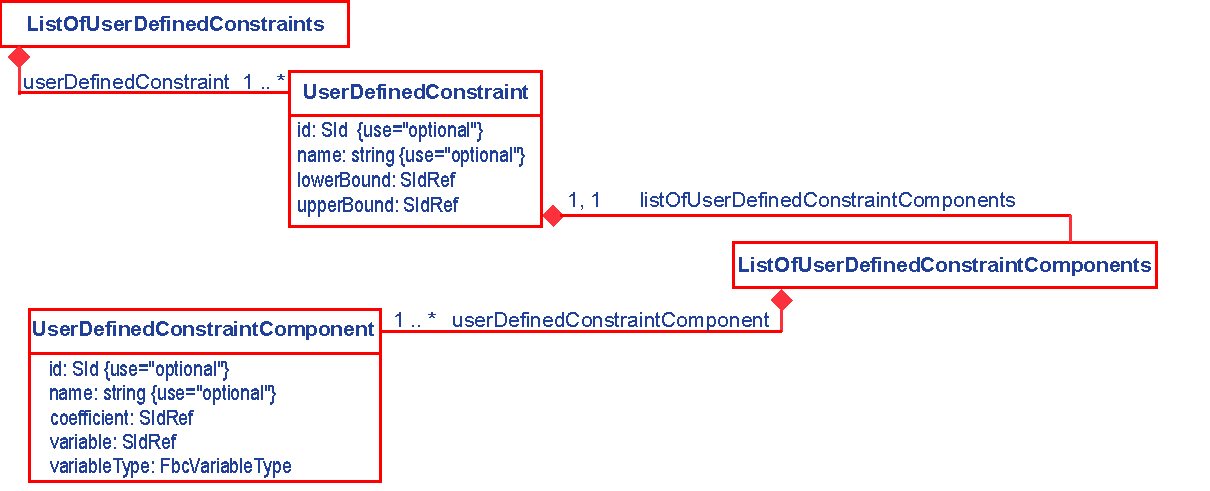
\includegraphics[width=0.9\textwidth]{images/fbc_v3_uml_userdefinedconstraint.pdf}\\
  \caption{A UML representation of the \SBML \Model class extended in
  the \FBCPackage by the \ListOfUserDefinedConstraints. See \ref{conventions} for conventions related to this figure.}
  \label{fig:fbc_v3_uml_user_constraints}
\end{figure}


\newtxt{Analogous to the attributes described in the \Reaction class (\ref{reaction-class-ga}), the \token{lowerBound} and \token{upperBound} define the upper and lower bounds of the \UserDefinedConstraint, such that:}
%
\begin{equation}\label{eqn:userderfinedconstraint}
\centering
  \token{lowerBound} \leq \UserDefinedConstraint \leq \token{upperBound}
\end{equation}

%
\newtxt{The \UserDefinedConstraint contains a \ListOfUserDefinedConstraintComponents representing a linear combination of \UserDefinedConstraintComponent{s}. Similar to a \FluxObjective each \UserDefinedConstraintComponent contains a coefficient--variable pair where the \token{coefficient} refers to a constant \Parameter. Furthermore, the \UserDefinedConstraintComponent \token{variable} attribute may either refer to a \Reaction or to a non-constant \Parameter, thus allowing the use of non-reaction, artificial, variables. See the attribute descriptions for more detail.}

\paragraph{The \token{id} and \token{name} attributes}
\newtxt{A \UserDefinedConstraint has an optional \token{id} of type
\primtype{SId} and an optional attribute \token{name} of type \primtype{string}.}

\paragraph{The \token{lowerBound} attribute}
\newtxt{The required \token{lowerBound} attribute contains an \primtype{SIdRef} that references a \Parameter which contains the lower boundary value of the \UserDefinedConstraint.}

\paragraph{The \token{upperBound} attribute}
\newtxt{The required \token{upperBound} attribute contains an \primtype{SIdRef} that references a \Parameter which contains the upper boundary value of the \UserDefinedConstraint.}

\paragraph{The \token{listOfUserDefinedConstraintComponents} element}
\label{listofuserdefinedconstraintcomponents-class}

\newtxt{The element \token{listOfUserDefinedConstraintComponents} which contains a
\ListOfUserDefinedConstraintComponents is derived from and functions like a typical \SBML
\textsf{\textbf{ListOf\rule{0.15in}{0.5pt}}} class with the restriction that it
must contain one or more elements of type \UserDefinedConstraintComponent (see \ref{userdefinedconstraintcomponent-class}).This implies that if a \UserDefinedConstraint is defined there should be at least one \UserDefinedConstraintComponent contained in a \ListOfUserDefinedConstraintComponents.}

\subsection{The \FBC \class{UserDefinedConstraintComponent} class}
\label{userdefinedconstraintcomponent-class}

\newtxt{The \FBC \UserDefinedConstraintComponent class is derived from \SBML \SBase and inherits
\token{metaid} and \token{sboTerm}, as well as the subcomponents for
\Annotation and \Notes. The \UserDefinedConstraintComponent class is a relatively simple container for a variable and a variable type specifier which is weighted by a signed coefficient.}

\paragraph{The \token{id} and \token{name} attributes}
\newtxt{An \UserDefinedConstraintComponent has an optional \token{id} of type \primtype{SId} and an optional attribute \token{name} of type \primtype{string}.}

\paragraph{The \token{coefficient} attribute}
\newtxt{The required \token{coefficient} attribute contains an \primtype{SIdRef} that is restricted to reference only a \Parameter which holds the coefficient value. In \textbf{strict} mode a \Parameter whose \primtype{SId} is referenced by a \token{coefficient}, has to be set as \token{constant} and not take the value \val{NaN} or \val{$\pm$INF}.}

\paragraph{The \token{variable} attribute}
\newtxt{The required \token{variable} attribute contains an \primtype{SIdRef} that is restricted to reference the \primtype{SId} of either a \Reaction or non-constant \Parameter. In \textbf{strict} mode such a non-constant \Parameter whose \primtype{SId} is referenced by a \UserDefinedConstraintComponent \token{variable} attribute may not be referenced by any \UserDefinedConstraintComponent \token{coefficient}, \UserDefinedConstraint \token{lowerBound} \& \token{upperBound} or \Reaction \token{lowerFluxBound} \& \token{upperFluxBound} attribute.}

\paragraph{The \token{variableType} attribute}
\newtxt{The required \token{variableType} attribute contains a \primtype{FbcVariableType} that indicates whether a variable should be considered as \val{linear} or \val{quadratic}.}

\paragraph{An example of encoding two user defined constraints in \SBML}
\newtxt{The following example illustrates the encoding of two \UserDefinedConstraint{s}. The first uses only \Reaction{s} as variables, while the second introduces an artificial, non-constant, \Parameter as a variable.}
\begin{eqnarray}
% \nonumber to remove numbering (before each equation)
  RGLX - RBTK  &=& 5 \\
  2\cdot p1var - RGDP &\geq& 2
\end{eqnarray}
\exampleFile{examples/ex-v3-userdefinedconstraints.txt}

\newpage
\subsection{The \FBC \class{ListOfKeyValuePairs} class}
\label{listofkeyvaluepairs-class}

\newtxt{The \ListOfKeyValuePairs, see \ref{fig:fbc_v3_uml_keyvalue} for details, forms the basis of a controlled annotation defined by the \FBCPackage. This element defines a `descriptive list' data keys and associated values which can be used to store metadata that is not encodable as a typical \SBML \Annotation.}
%
\exampleFile{examples/ex-v3-kvp1.txt}
%
\newtxt{As such it is analogous, and supplemental, to the official \SBML RDF annotation used to support MIRIAM compliant annotations defined in the \SBML specification. The \ListOfKeyValuePairs is an element of an \Annotation that declares the \token{xmlns} attribute to be \token{http://sbml.org/fbc/keyvaluepair} and then strictly applies the \ListOfKeyValuePairs format. As it is defined as an \Annotation, software may choose to support reading and interpreting the \ListOfKeyValuePairs content and optionally ignore the annotation and merely read and write it with any other third party \Annotation{s}. However, as is the case with the RDF/MIRIAM \Annotation{s}, read and write support for \ListOfKeyValuePairs will be included in the \SBML support libraries and be easily accessible to tool developers.}
%
\begin{figure}[ht]
  \centering
  % Requires \usepackage{graphicx}
  %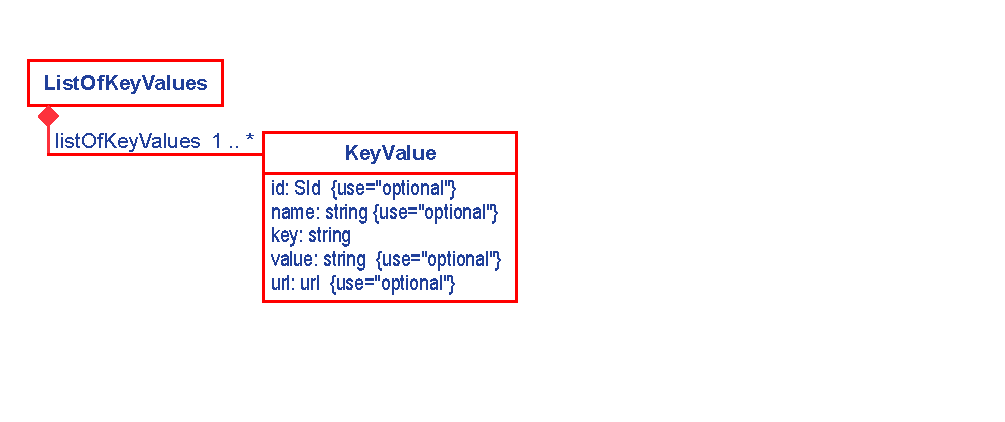
\includegraphics[width=6cm]{images/fbc_v3_uml_keyvalue.pdf}\\
  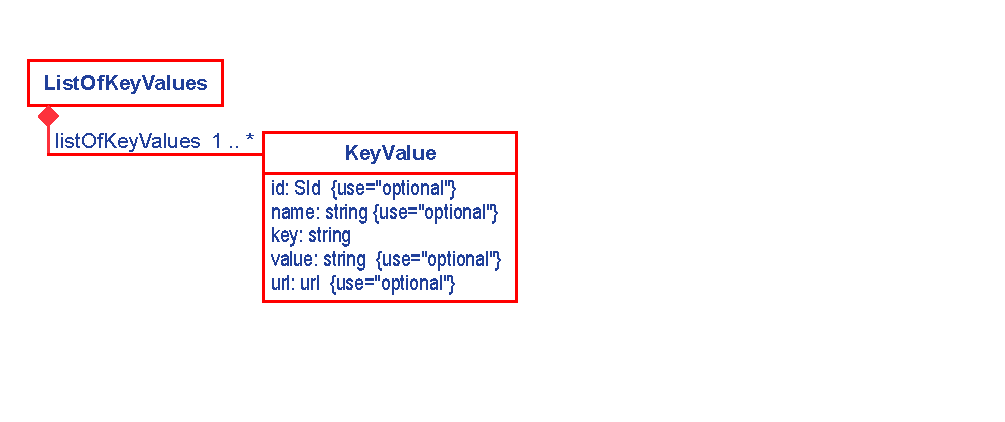
\includegraphics[width=0.6\textwidth]{images/fbc_v3_uml_keyvalue.pdf}\\
  \caption{A UML representation of the \SBML \SBase class extended in
  the \FBCPackage by the \protect{\ListOfKeyValuePairs}. See \ref{conventions} for conventions related to this figure.}
  \label{fig:fbc_v3_uml_keyvalue}
\end{figure}

\newtxt{The \ListOfKeyValuePairs functions like a typical \SBML \textsf{\textbf{ListOf\rule{0.15in}{0.5pt}}} class with the restriction that it must contain one or more elements of type \KeyValuePair (see \ref{keyvaluepair-class}). In addition it defines a single mandatory attribute, \token{xmlns}, which identifies the annotation as belonging to the \FBCPackage.}

\paragraph{The \token{xmlns} attribute}
\newtxt{The \token{xmlns} is a mandatory component of the \ListOfKeyValuePairs of type \primtype{uri}. It takes a single value: \token{http://sbml.org/fbc/keyvaluepair}.}


\subsection{The \FBC \class{KeyValuePair} class}
\label{keyvaluepair-class}

\newtxt{The \FBC \KeyValuePair class defines a typical key--value pair and includes single, mandatory attribute, the \token{key}, as well as four optional attributes: \token{value}, \token{uri}, \token{id} and \token{name}.}

\paragraph{The \token{id} and \token{name} attributes}
\newtxt{A \KeyValuePair defines two optional attributes: \token{id} an attribute of
type \primtype{SId} and \token{name} of type \primtype{string}.}

\paragraph{The \token{key} attribute}
\newtxt{The \token{key} is the mandatory component of the \KeyValuePair pair and is of type \primtype{string}. It has the special property that every \token{key} in an enclosing \ListOfKeyValuePairs must be unique.}

\paragraph{The \token{value} attribute}
\newtxt{The optional \token{value} attribute is of \primtype{string} and contains the matching \token{value} associated with a particular \token{key}. If not present, the \KeyValuePair is defined as having no value.}

\paragraph{The \token{uri} attribute}
\newtxt{The optional attribute \token{uri} is of type \primtype{uri}. The \token{uri} points to a resource that defines the meaning of the \token{key} component of the \KeyValuePair, see~\ref{table:kvpuris} for examples of the types of values a \token{uri} may take. As a best practice, it is highly recommended that tools implementing a \KeyValuePair also implement support for the \token{uri} attribute.}
%
\begin{table}[h]
  \centering
  \begin{tabular}{lll}
  \toprule
   \textbf{Type} & \textbf{Example} & \textbf{Description} \\
  \midrule
   \textbf{urn} & urn:awesometool.com:keyvaluepair & a tool specific namespace declaration \\
   \textbf{url} & \url{https://github.com/awesometool/keyvaluepair.md} & a \textbf{url} containing a set of \token{key} definitions\\
   \bottomrule
  \end{tabular}
   \caption{Examples of how the \token{uri} attribute can be used to identify \token{key} definitions by way of a \textbf{urn} or \textbf{url}.}\label{table:kvpuris}
\end{table}

%%%%%%%%%%%%%%%%%%%%%%%%%%%%%%%%%%%%%%%%%%%%%%%%%%%%%%%%%%%%%%%%%%%%%%%%
% Original FBC text as developed by the FBC community - can be deleted %
%%%%%%%%%%%%%%%%%%%%%%%%%%%%%%%%%%%%%%%%%%%%%%%%%%%%%%%%%%%%%%%%%%%%%%%%

%\newpage
%\section{\FBC version 3: updated HARMONY 2020}

%The proposed \FBCPackage version~3 extends the definition of the \FluxObjective, extends the definition of the \token{chemicalFormula}, redefines \token{charge} as a double, defines a \UserDefinedConstraint and adds a generic \KeyValuePair annotation.
%
%\begin{quote}
% \newtxt{\textbf{The extensions and modifications contained in this document are proposed as version 3 of the \FBCPackage. This proposal is been formulated through open discussions on the \FBC PWG mailing list and intense discussion during HARMONY 2018 and HARMONY 2020. }}
%\end{quote}
%%
%\begin{quote}
%  \newtxt{At HARMONY 2020 it was decided that the name `UserDefinedConstraint' should be changed to something else.}
%\end{quote}
%
%%
%Please note that where specification text (or UML) has been modified and diverges from the \FBCPackage version~2 specification, it has been colored \newtxt{red}.
%
%\begin{figure}[ht!]
%  \centering
%  % Requires \usepackage{graphicx}
%  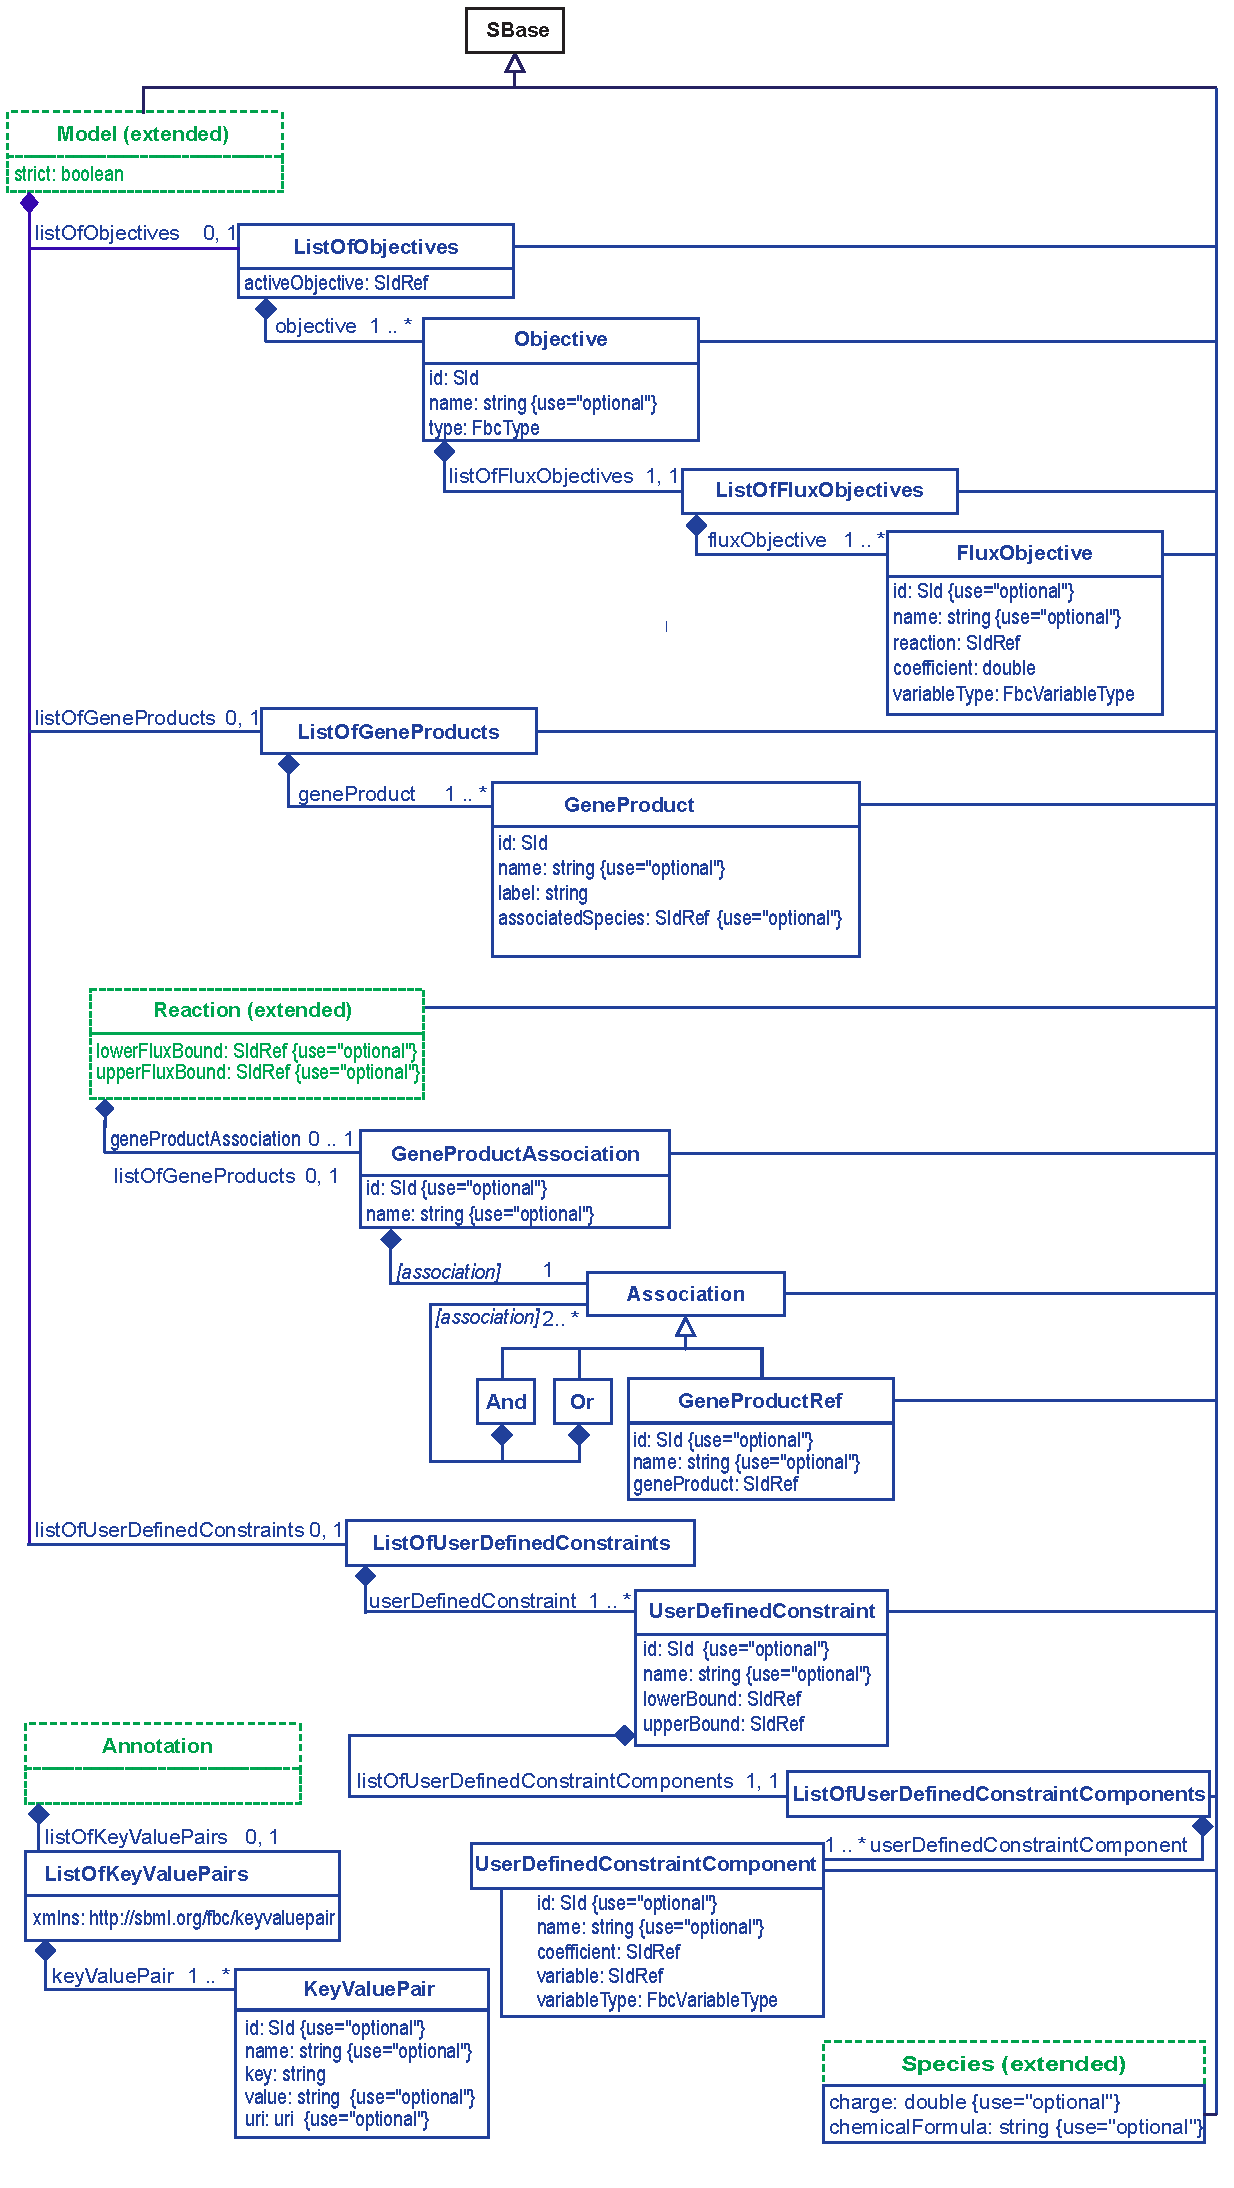
\includegraphics[height=0.85\textheight]{images/fbc_uml_v3.pdf}\\
%  \caption{A UML representation of the \FBCPackage version three. Derived from \SBase, most\FBC classes inherit support for constructs such as SBML \Notes and \Annotation's. The [association] element name is the name of the class, de-capitalized. In this case, the possible values are "and", "or", or "geneProductRef". See \ref{conventions} for conventions related to this figure. The individual classes are further discussed in the text.}
%  \label{fig:fbc_uml_v3}
%\end{figure}

%\subsection{The extended \class{SBase} class}
%\label{sbase-class-kv}

%\subsection{The extended \class{Model} class (updates specification \ref{model-class})}
%\label{model-class-kv}
%\label{listoffluxbounds-class}



%\subsubsection{Type \primtypeNC{FbcVariableType}}
%\label{primtype-fbcvariabletype}
%
%The \FBCPackage defines a new enumerated type \primtype{FbcVariableType} which
%represents the index of a variable that occurs in either the \FluxObjective or \UserDefinedConstraintComponent. It contains the following two values, \val{linear} or \val{quadratic}.


%\subsubsection{Type \primtypeNC{FbcUCCVariableType}}
%\label{primtype-fbcuserdefinedconstraintvariabletype}
%
%The \FBCPackage defines a new enumerated type \primtype{FbcUCCVariableType} which
%represents the index of a variable that occurs in a user defined constraint. It can have one
%of the following two values \val{linear} or \val{quadratic}.

%The \SBML \Model class is extended by a \token{listOfUserDefinedConstraints} of which it may contain at most one, see  \ref{fig:fbc_v3_uml_user_constraints}.
%
%\subsubsection{The \FBC \class{listOfUserDefinedConstraints}}
%\label{listofuserdefinedconstraints-class}
%
%As shown in \ref{fig:fbc_v3_uml_user_constraints} the \ListOfUserDefinedConstraints is derived from \SBase and inherits the attributes \token{metaid} and \token{sboTerm}, as well as
%the subcomponents for \Annotation and \Notes. The \ListOfUserDefinedConstraints must contain at least one \UserDefinedConstraint (defined in \ref{userdefinedconstraint-class}).

%\pagebreak
%
%\subsection{The extended \class{Species} class (updates specification \ref{species-class})}
%
%The \FBCPackage extends the \sbmlthreecore \Species class with the addition
%of two attributes \token{charge} and \token{chemicalFormula}.
%%
%\begin{figure}[h]
%  \centering
%  % Requires \usepackage{graphicx}
%  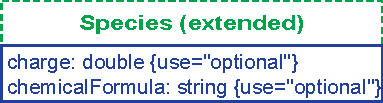
\includegraphics[width=6cm]{images/v3harmony_fbc_species.pdf}\\
%  \caption{A UML representation of the extended \SBML \Species class used in
%  the \FBCPackage. See \ref{conventions} for conventions related to this
%  figure.}
%  \label{fig:fbc_uml_species_v3}
%\end{figure}

%\paragraph{The \token{charge} attribute}
%
%\newtxt{The optional attribute charge contains a signed double referring to the Species object’s charge (in terms of electrons, not the SI unit coulombs). Note, that unlike FBC versions one and two a \Species may, for the purposes of charge, be interpreted as a pseudoisomer or aggregate molecule and may assume a non-integer value. Non-integer charges should be used with caution as their use may have unintended side-effects, for example, with respect to the accuracy of reaction balancing.}
%
%%The optional attribute \token{charge} which contains a signed
%%\primtype{integer} referring to the \Species object's charge and is
%%defined as it was in the \SBML Level 2 Version 1 specification
%%: \textit{``The optional field charge takes an integer indicating
%%the charge on the species (in terms of electrons, not the SI unit coulombs).''}
%
%\paragraph{The \token{chemicalFormula} attribute}
%\label{chemicalFormula-attribute}
%
%The optional attribute \token{chemicalFormula} containing a \primtype{string} that represents the \Species objects elemental composition.
%%
%\exampleFile{examples/ex-v3-species.txt}
%%
%\newtxt{While there are many ways of referring to an elemental composition, the purpose of the \token{chemicalFormula} attribute is to enable reaction balancing and validation, something of particular importance in constraint-based models.}
%
%\newtxt{The format of the \token{chemicalFormula} should, whenever possible, consist only of atomic names
%(as in the Periodic Table). Similarly, for enhanced inter-operability, the element order should be arranged according to the Hill system (see \ref{table:hill2})} \citep{hillsystem, hillwikipedia}.
%%
%\begin{table}[h!]
%  \begin{tabular}{ccc}
%    % after \\: \hline or \cline{col1-col2} \cline{col3-col4} ...
%     $H_{2}O_{4}S$ & $C_{2}H_{5}Br$ & $BrH$ \\
%     $C_{10}H_{12}N_{5}O_{13}P_{3}$ & $CH_{3}I$ & $CH_{4}$  \\
%  \end{tabular}
%  \caption{Examples of chemical formulas written using the Hill System. As
%	described in \ref{chemicalFormula-attribute}}\label{table:hill2}
%\end{table}
%%
%\newtxt{Using this notation the number of carbon atoms in a molecule is indicated first, followed by the number of hydrogen atoms and then the number of all other chemical elements in alphabetical order. When the formula contains no carbon; all elements, including hydrogen, are listed alphabetically. Where there is more than a single atom present, this is indicated with an integer that follows the element symbol.}
%
%\newtxt{However, in certain situations it does become necessary to use a generic symbol in a user defined compound. For example, such symbols can include \textsf{R} and \textsf{X} and have the general form of a single capital letter followed by zero or more lowercase letters.}
%%
%\begin{table}[h!]
%  \begin{tabular}{ccc}
%    % after \\: \hline or \cline{col1-col2} \cline{col3-col4} ...
%     $RCONH_{2}$ & $RCOX$ & $C_{2}H_{4}O_{2}(CH_{2})_{n}$ \\
%  \end{tabular}
%  \caption{Examples of chemical formulas written using allowed non-Hill symbols, as described in \ref{chemicalFormula-attribute}.}\label{table:non-hill}
%\end{table}
%%
%\newtxt{In addition, the undefined parenthesised group index $(\ldots)_n$ may also be used. Note that in this case only the subscript $n$ is allowed, integer values $(\ldots)_2$ and expressions such as $(\ldots)_{n-1}$ are considered invalid.}
%
%\newtxt{However, the use of \textsf{R}, \textsf{X} and $(\ldots)_n$ is not advised, as any \Reaction in which such a \Species occurs cannot necessarily be balanced. Therefore, any \token{chemicalFormula} that contains any of the aforementioned, non-Hill compatible symbols will raise a `best practices' warning on model validation.}

%\subsection{The \FBC \class{FluxObjective} class}
%
%The \FBC \FluxObjective class is derived from \SBML \SBase and inherits
%\token{metaid} and \token{sboTerm}, as well as the subcomponents for
%\Annotation and \Notes.
%%
%\begin{figure}[ht]
%  \centering
%  % Requires \usepackage{graphicx}
%  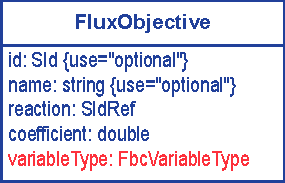
\includegraphics[width=6cm]{images/fbc_v3_uml_fobj.pdf}\\
%  \caption{A UML representation of the \FBCPackage \FluxObjective class. For a complete description see \ref{fig:fbc_uml} as well as \ref{conventions} for conventions related to this figure.}
%  \label{fig:fbc_uml_userdefinedconstraint}
%\end{figure}
%%
%The \FluxObjective class is a relatively simple container for a model
%variable that can be expressed as a `linear' or `quadratic', weighted by a signed linear coefficient.
%
%\paragraph{The \token{id} and \token{name} attributes}
%A \FluxObjective has two optional attributes: \token{id} an attribute of
%type \primtype{SId} and \token{name} an attribute of type \primtype{string}.
%
%\paragraph{The \token{reaction} and \token{coefficient} attributes}
%The required \token{reaction} is of type \primtype{SIdRef} and is restricted
%to refer only to a \Reaction while the \token{coefficient} attribute
%holds a \primtype{double} referring to the coefficient that this \FluxObjective
%takes in the enclosing \Objective.
%
%\newtxt{\paragraph{The \token{variableType} attribute}
%The required \token{variableType} attribute contains a \primtype{FbcVariableType} that
%represents the index to which a variable is raised in a \FluxObjective. For example, where $J_{x}$ represents a steady-state flux the \primtype{FbcVariableType} defines either a \val{linear}, $J^1_x$ or \val{quadratic}, $J^2_x$ term.}
%
%\paragraph{Flux objectives: example code}
%\newtxt{An objective with purely linear terms in LP format:} \verb"Maximize: 1 R1 + 2 R2"
%%
%\exampleFile{examples/ex-v3-fluxobjective-linear.txt}
%%
%\newtxt{Similarly, an objective with a quadratic term in LP format:} \verb"Minimize: 1 R1 + [4 R2^2]/2"
%%
%\exampleFile{examples/ex-v3-fluxobjective.txt}
%
%\paragraph{Units}
%As described above the linear \FluxObjective defined here as $n\cdot J$ where
%the \token{coefficient} ($n$) is dimensionless and the \token{value} ($J$)
%takes the units of the \token{reaction} flux i.e.,~``extent per time''.
%\newtxt{Therefore, the \token{linear} \FluxObjective, ($n\cdot J$)  has the unit $\frac{extent}{time}$ where the units of reaction ``extent'' and ``time'' are defined globally. Analogously, in the case of a \token{quadratic} \FluxObjective, $n\cdot J^{2}$ this would be $\frac{extent^{2}}{time^{2}}$}.



%\subsection{The \FBC \class{UserDefinedConstraint} class}
%\label{userdefinedconstraint-class}
%
%The \FBC \UserDefinedConstraint class is derived from \SBML \SBase and inherits
%\token{metaid} and \token{sboTerm}, as well as the subcomponents for
%\Annotation and \Notes. It's purpose is to define non-stoichiometric constraints, that is  constraints that are not necessarily defined by the stoichiometrically coupled reaction network. In order to achieve we defined a new type of linear constraint, the \UserDefinedConstraint.
%%
%\begin{figure}[ht]
%  \centering
%  % Requires \usepackage{graphicx}
%  %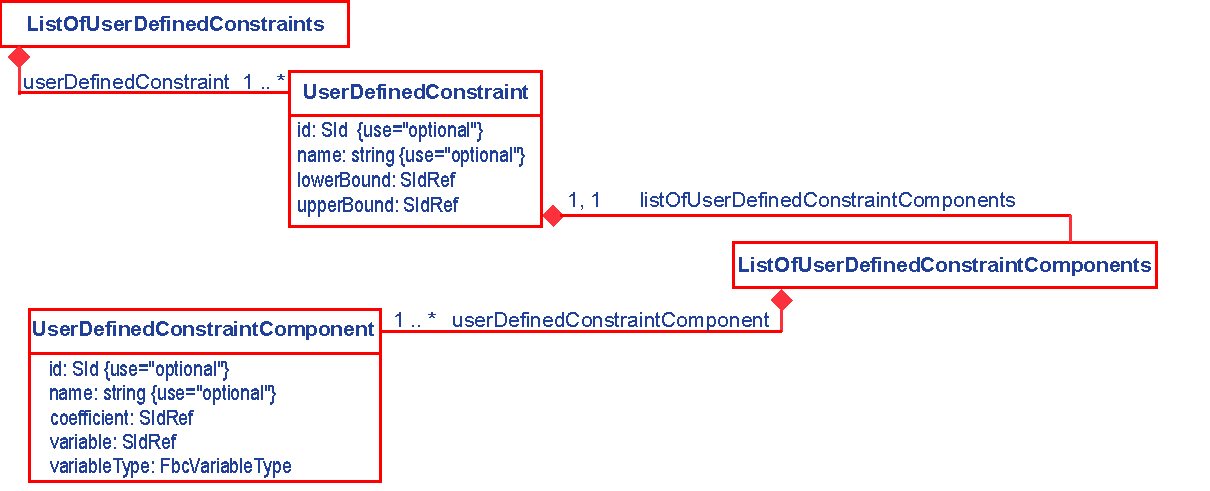
\includegraphics[width=6cm]{images/fbc_v3_uml_userdefinedconstraint.pdf}\\
%  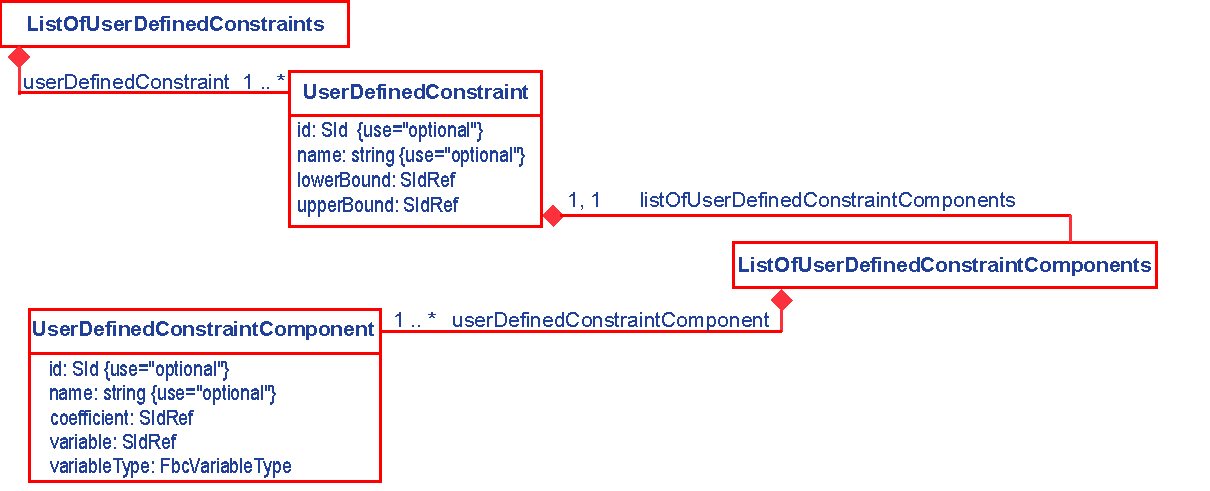
\includegraphics[width=0.9\textwidth]{images/fbc_v3_uml_userdefinedconstraint.pdf}\\
%  \caption{A UML representation of the \SBML \Model class extended in
%  the \FBCPackage by the \ListOfUserDefinedConstraints. See \ref{conventions} for conventions related to this figure.}
%  \label{fig:fbc_v3_uml_user_constraints}
%\end{figure}
%
%
%Analogous to the attributes described in \ref{reaction-class-ga} the \token{lowerBound} and \token{upperBound} form the boundaries of the \UserDefinedConstraint.
%%
%\begin{eqnarray}
%% \nonumber to remove numbering (before each equation)
%  \UserDefinedConstraint &=& \token{value} \\
%  \UserDefinedConstraint &\geq& \token{lowerBound value} \\
%  \UserDefinedConstraint &\leq& \token{upperBound value}
%\end{eqnarray}
%%
%Defining either an equality if both \token{lowerBound} and \token{upperBound} refere to the same parameter (Equation~4) or set of inequalities (Equations 4 and 5).
%
%The \UserDefinedConstraint contains a \ListOfUserDefinedConstraintComponents representing a linear combination of \UserDefinedConstraintComponent{s}. Similar to a \FluxObjective each \UserDefinedConstraintComponent contains a coefficient--variable pair where the \token{coefficient} refers to a \Parameter. In addition to a \Reaction a \UserDefinedConstraintComponent allows the \token{variable} to refer to non-constant \Parameter thus allowing the definition of non-reaction, artificial, variables.
%
%\paragraph{The \token{id} and \token{name} attributes}
%A \UserDefinedConstraint has an optional \token{id} of type
%\primtype{SId} and an optional attribute \token{name} of type \primtype{string}.
%
%\paragraph{The \token{lowerBound} attribute}
%The required \token{lowerBound} attribute contains an \primtype{SIdRef} that references a \Parameter which contains the lower boundary value of the \UserDefinedConstraint.
%
%\paragraph{The \token{upperBound} attribute}
%The required \token{upperBound} attribute contains an \primtype{SIdRef} that references a \Parameter which contains the upper boundary value of the \UserDefinedConstraint.
%
%\paragraph{The \token{listOfUserDefinedConstraintComponents} element}
%\label{listofuserdefinedconstraintcomponents-class}
%
%The element \token{listOfUserDefinedConstraintComponents} which contains a
%\ListOfUserDefinedConstraintComponents is derived from and functions like a typical \SBML
%\textsf{\textbf{ListOf\rule{0.15in}{0.5pt}}} class with the restriction that it
%must contain one or more elements of type \UserDefinedConstraintComponent (see \ref{userdefinedconstraintcomponent-class}).
%This implies that if a \UserDefinedConstraint is defined there should be at least
%one \UserDefinedConstraintComponent contained in a \ListOfUserDefinedConstraintComponents.
%
%\subsection{The \FBC \class{UserDefinedConstraintComponent} class}
%\label{userdefinedconstraintcomponent-class}
%
%The \FBC \UserDefinedConstraintComponent class is derived from \SBML \SBase and inherits
%\token{metaid} and \token{sboTerm}, as well as the subcomponents for
%\Annotation and \Notes. The \UserDefinedConstraintComponent class is a relatively simple container for a variable and a variable type specifier which is weighted by a signed coefficient.
%
%\paragraph{The \token{id} and \token{name} attributes}
%An \UserDefinedConstraintComponent has an optional \token{id} of type \primtype{SId} and an optional attribute \token{name} of type \primtype{string}.
%
%\paragraph{The \token{coefficient} attribute}
%The required \token{coefficient} attribute contains an \primtype{SIdRef} that is restricted to reference only a constant \Parameter which holds the coefficient value. In \textbf{strict} mode a \Parameter whose \primtype{SId} is referenced by a \token{coefficient}, as in the case of a \FluxObjective \token{coefficient}, has to be constant and not take the value NaN or $\pm$inf.
%
%\paragraph{The \token{variable} attribute}
%The required \token{variable} attribute contains an \primtype{SIdRef} that is restricted to reference the \primtype{SId} of either a \Reaction or a non-constant \Parameter. Conversely, if such non-constant \Parameter's \primtype{SId} is referenced by a \UserDefinedConstraintComponent's \token{variable} attribute it may not be referenced by any \token{coefficient}, \token{lowerFluxBound} or \token{upperFluxBound} attribute.
%
%\paragraph{The \token{variableType} attribute}
%The required \token{variableType} attribute contains a \primtype{FbcVariableType} that indicates whether a variable should be considered as `linear' or `quadratic'.
%
%\paragraph{User constraints: example code}
%The following example illustrates the encoding of the following two \UserDefinedConstraint{s}:
%\begin{eqnarray}
%% \nonumber to remove numbering (before each equation)
%  RGLX - RXLG  &=& 5 \\
%  2\cdot Avar - RGDP &\geq& 2
%\end{eqnarray}
%\exampleFile{examples/ex-v3-userdefinedconstraints.txt}





%\subsection{The \FBC \class{ListOfKeyValuePairs} class}
%\label{listofkeyvaluepairs-class}
%
%The \ListOfKeyValuePairs, see \ref{fig:fbc_v3_uml_keyvalue} for details, forms the basis of a controlled annotation defined by the \FBCPackage. This element defines a `structured note' or `descriptive list' of keys and associated values.
%%
%\exampleFile{examples/ex-v3-kvp1.txt}
%%
%As such it is analogous to the official \SBML RDF annotation used to support MIRIAM annotations, as defined in the \SBML specification documents. When an annotation that declares the \token{xmlns} \token{http://sbml.org/fbc/keyvaluepair} then it must have the format specified here. Tools may choose to support reading and interpreting the content as described, but may optionally ignore the annotation and merely round trip it with any other third party annotations. As is the case with the RDF/MIRIAM annotations, support for \ListOfKeyValuePairs will be included in the \SBML support libraries.
%%
%\begin{figure}[ht]
%  \centering
%  % Requires \usepackage{graphicx}
%  %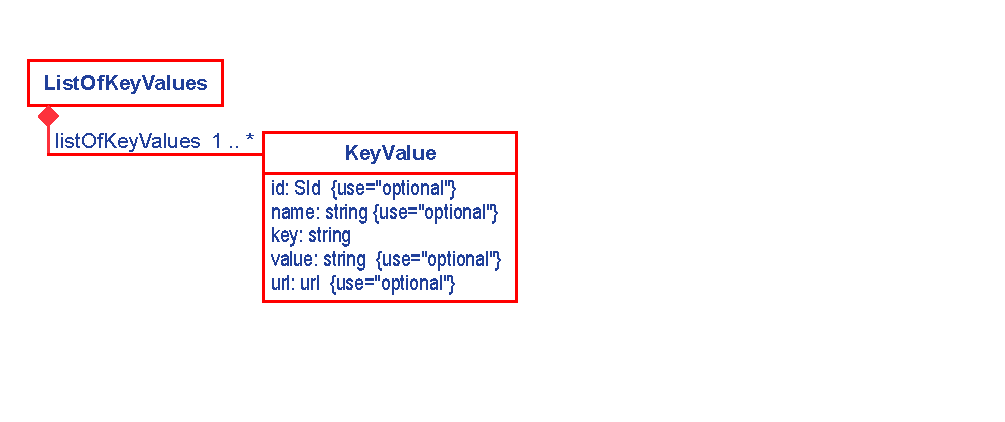
\includegraphics[width=6cm]{images/fbc_v3_uml_keyvalue.pdf}\\
%  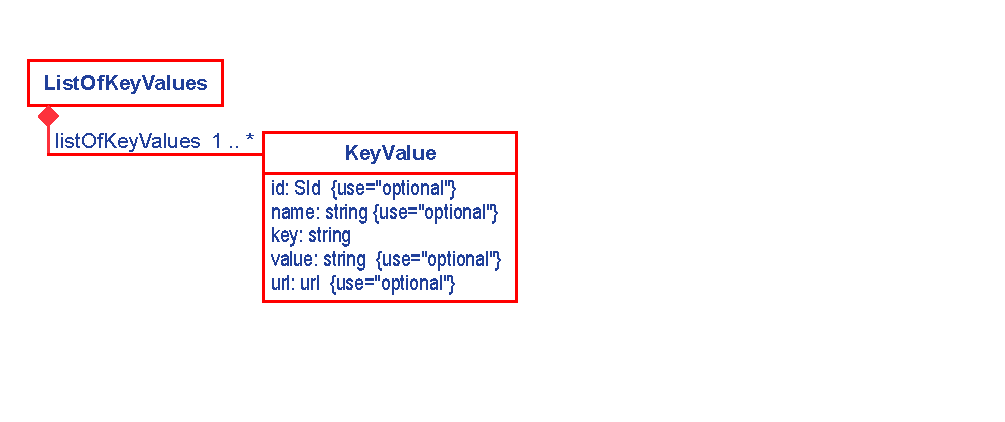
\includegraphics[width=0.6\textwidth]{images/fbc_v3_uml_keyvalue.pdf}\\
%  \caption{A UML representation of the \SBML \SBase class extended in
%  the \FBCPackage by the \protect{\ListOfKeyValuePairs}. See \ref{conventions} for conventions related to this figure.}
%  \label{fig:fbc_v3_uml_keyvalue}
%\end{figure}
%%
%The \ListOfKeyValuePairs functions like a typical \SBML \textsf{\textbf{ListOf\rule{0.15in}{0.5pt}}} class with the restriction that it must contain one or more elements of type \KeyValuePair (see \ref{keyvaluepair-class}). In addition it defines a single mandatory attribute, \token{xmlns}, which identifies the annotation as belonging to the \FBCPackage.
%
%\paragraph{The \token{xmlns} attribute}
%The \token{xmlns} is a mandatory component of the \ListOfKeyValuePairs, is of the type \primtype{uri} and must have the value \token{http://sbml.org/fbc/keyvaluepair}.
%
%
%\subsection{The \FBC \class{KeyValuePair} class}
%\label{keyvaluepair-class}
%
%The \FBC \KeyValuePair class' sole purpose is to define a key--value pair with an optional extended key definition.
%
%The \KeyValuePair defines a single mandatory attribute the \token{key} as well as four optional attributes: \token{value}, \token{uri}, \token{id} and \token{name}.
%
%\paragraph{The \token{id} and \token{name} attributes}
%A \KeyValuePair has two optional attributes: \token{id} an attribute of
%type \primtype{SId} and \token{name}, an attribute of type \primtype{string}.
%
%\paragraph{The \token{key} attribute}
%The \token{key} is the mandatory component of the \KeyValuePair pair and is of type \primtype{string}. It has the special property that every \token{key} in an enclosing \ListOfKeyValuePairs must be unique.
%
%\paragraph{The \token{value} attribute}
%The optional \token{value} attribute is of \primtype{string} and contains the value associated with a particular \token{key}. If not present, the \KeyValuePair is defined as having no value.
%
%\paragraph{The \token{uri} attribute}
%The optional attribute \token{uri} is of type \primtype{uri}. This attribute identifies a resource that defines the associated \token{key} component of the \KeyValuePair, see~\ref{table:kvpuris} for examples. As a best practice, it is highly recommended that all tools implementing a \KeyValuePair also implement support for the \token{uri} attribute.
%%
%\begin{table}
%  \centering
%  \begin{tabular}{lll}
%  \toprule
%   \textbf{Type} & \textbf{Example} & \textbf{Description} \\
%  \midrule
%   \textbf{urn} & urn:tinyurl.com:example:kvp & a tool specific namespace declaration \\
%   \textbf{url} & \url{https://tinyurl.com/ybyr7b62} & a url identifying a set of \token{key} definitions\\
%   \bottomrule
%  \end{tabular}
%   \caption{Examples of how the \token{uri} attrbitue can be used to identify \token{key} definitions by \textbf{urn} or \textbf{url}.}\label{table:kvpuris}
%\end{table}





